\documentclass[letterpaper,10pt]{book}
\usepackage{cergtheme}
\usepackage{afterpage}
\usepackage{amsmath,amssymb,latexsym,amsthm,amsfonts}
\usepackage[utf8]{inputenc}
\usepackage[table,svgnames,dvipsnames]{xcolor}%for coloring the cells and rows
%\usepackage{multirow}
\usepackage{fancyvrb}
\usepackage{verbatim}
\usepackage{tcolorbox}

\usepackage{graphicx,rotating}
\usepackage{enumerate}%enumerating with roman, alpha etc.
\usepackage{array,multirow}
\usepackage{multicol}
\usepackage{xcolor}
\usepackage{color}
%\usepackage[framed,numbered,autolinebreaks,useliterate]{mcode}%adding file as fgiures
%\usepackage{longtable}% for long tables spanning across multiple pages
\usepackage{setspace}% for setting the line spacing
\usepackage{datetime}
\onehalfspacing
\usepackage{amsmath}
\usepackage{algorithmic}
\usepackage{algorithm}
\usepackage{fullpage}%Using the full page
\usepackage{capt-of}%enables using caption without use of figure or table environment
\usepackage[pdftitle=FOBOS-CERG,pdfauthor=Panasayya Yalla,pdffitwindow=true, pdfcreator=Panasayya Yalla,
            pdfsubject=SideChannel\ Power Analysis\ ,pdfkeywords={Side Channel, Cryptography, Power Analysis, DPA},
            colorlinks=false]{hyperref}%For linking tables and figures in the document.

%\usepackage[usenames,dvipsnames]{xcolor}
%opening
\renewcommand\familydefault{\rmdefault}
%%%%%setting for table boaders%%%%%
\setlength{\arrayrulewidth}{0.5mm}
\setlength{\tabcolsep}{18pt}
\renewcommand{\arraystretch}{1.0}% for streching the tables
%%%%%%%%%%%%%%%%%%%%%%%%%%%%%%%%%%%%%%%%%%%%%%%%%%
\usepackage{glossaries}
%\makeglossaries
\makeglossaries
%%%%%%%%%%%%%%%%%%%%%%%%%%%%%%%%%%%
% redefine \VerbatimInput
\RecustomVerbatimCommand{\VerbatimInput}{VerbatimInput}%
{fontsize=\footnotesize,
	%
	frame=lines,  % top and bottom rule only
	framesep=2em, % separation between frame and text
	rulecolor=\color{Gray},
	%
	%label=\fbox{\color{Black}data.txt},
	%labelposition=topline,
	%
	commandchars=\|\(\), % escape character and argument delimiters for
	% commands within the verbatim
	commentchar=*        % comment character
}





%%%%%%%%SETTING THE TITLE PAGE%%%%%%%%%%%%%%5
\usepackage{pdfcolmk}
%\pdftitle={Interface-CERG}
%\usepackage[svgnames]{xcolor}

%%%%%%%%%%%%%%%%%%Drawing folder structure
\usepackage{tikz}
\usetikzlibrary{trees}
%%%%%%%%%%%%%%%%%%%%%%%%%%%%%%%%%%%%%%%%%%%%%%%%%%%%%
%----------------------------------------------------------------------------------------
%   TITLE PAGE
%----------------------------------------------------------------------------------------
\newlength{\drop} % Command for generating a specific amount of whitespace
\newcommand*{\titleAT}
    {
    \begingroup % Create the command for including the title page in the document
    \centering % Center all text
    \drop=0.1\textheight % Define the command as 10% of the total text height
    \rule{\textwidth}{1pt}\par % Thick horizontal line
    \vspace{2pt}\vspace{-\baselineskip} % Whitespace between lines
    \rule{\textwidth}{0.4pt}\par % Thin horizontal line
    \vspace{0.25\drop} % Whitespace between the top lines and title
    
        \textcolor{black}
	{
            { \Huge \textbf{Flexible Opensource workBench }}\\
	    { \Huge \textbf{fOr}}\\
	    { \Huge \textbf{Side-channel analysis}}
    }    \\ 
        \drop=0.1\textheight % Define the command as 10% of the total text height
	\rule{\textwidth}{1pt}\par % Thick horizontal line
	\vspace{2pt}\vspace{-\baselineskip} % Whitespace between lines
	\rule{\textwidth}{0.4pt}\par % Thin horizontal line
	\vspace{0.25\drop} % Whitespace between the top lines and title
	{ \Large \textit{FOBOS User Guide $v1.0$}}\\
        %\title{FOBOS: A Prototype for Conducting Side-channel Evaluations on FPGAs}}\\[0.5\baselineskip] % Title line 1
        %\vspace{0.25\drop} % Whitespace between the title and short horizontal line
        %\rule{0.5\textwidth}{2.5pt}\par% Short horizontal line under the title
        %{\Huge{FOBOS Version 1.0}}\par
        \vspace{2.5\drop} % Whitespace between the thin horizontal line and the author name
        {\Large \textsc{Rajesh Velegalati, Panasayya Yalla \\ \& \\ Jens-Peter Kaps}}\\
        {\urlstyle{same}
		\nolinkurl{{rvelegal, pyalla, jkaps}'at'gmu.edu}} \par
            %{Email:\href{mailto:pyalla@gmu.edu}{pyalla@gmu.edu}}\par % Author name
        \vfill % Whitespace between the author name and publisher text
        %{\large \textcolor{Red}{\plogo}}\\[0.5\baselineskip] % Publisher logo
        {\large \textsc{George Mason University\\ Fairfax, Virginia}}\par % Publisher
                {\large \textit{ \today }}\par% Current date
        %{\large \textit{ October 15$^{th}$, 2015 }}\par% specific date
        %\vspace*{\drop} % Whitespace under the publisher text

        \begin{minipage}{\textwidth}
              \begin{minipage}[!t]{0.30\textwidth}
                \begin{center}
                     \vspace{1ex}
                    
\includegraphics[scale=0.35]{./themefigs/CERG-logo-sm.png}
                     % CERG-logo-sm.png: 200x150 pixel, 72dpi, 7.05x5.29 cm, bb=0 0 200 150
                \end{center}
            \end{minipage}
            \begin{minipage}[!t]{0.39\textwidth}
                 \hspace{3ex}
            \end{minipage}
            \begin{minipage}[!t]{0.30\textwidth}
		    \begin{center}    \begin{figure}
				    \centering
				    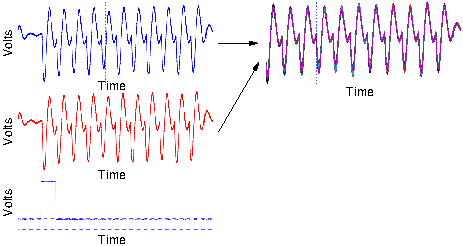
\includegraphics[scale=2.4]{../figures/tracealingment} 
			    \end{figure}
			
\includegraphics[scale=.50]{./themefigs/Mason-logo.png}
		\end{center}
            \end{minipage}
        \end{minipage}
        \rule{\textwidth}{0.4pt}\par % Thin horizontal line
        \vspace{2pt}\vspace{-\baselineskip} % Whitespace between lines
        \rule{\textwidth}{1pt}\par
        \begin{minipage}{\textwidth}
              \begin{minipage}[!t]{0.30\textwidth}
                \begin{center}
                     \vspace{1ex}
                    \href{https://cryptography.gmu.edu/}{www.cryptography.gmu.edu} % Thick horizontal line
                     % CERG-logo-sm.png: 200x150 pixel, 72dpi, 7.05x5.29 cm, bb=0 0 200 150
                \end{center}
            \end{minipage}
            \begin{minipage}[!t]{0.39\textwidth}
                 \hspace{3ex}
            \end{minipage}
            \begin{minipage}[!t]{0.30\textwidth}
		    \centering
                    \href{https://www.gmu.edu/}{www.gmu.edu} % Thick horizontal line
            \end{minipage}
        \end{minipage}
        %\href{http://cryptography.gmu.edu}{http://cryptography.gmu.edu} % Thick horizontal line
    \endgroup
    \clearpage
    \newcommand\blankpage{%
    \null
    \thispagestyle{empty}%
    \addtocounter{page}{-1}%
    \newpage}
    }
    
    
    \newcommand*{\titleATa}
        {
        \begingroup % Create the command for including the title page in the document
        \centering % Center all text
        \drop=0.1\textheight % Define the command as 10% of the total text height
        \rule{\textwidth}{1pt}\par % Thick horizontal line
        \vspace{2pt}\vspace{-\baselineskip} % Whitespace between lines
        \rule{\textwidth}{0.4pt}\par % Thin horizontal line
        \vspace{0.25\drop} % Whitespace between the top lines and title
        
            \textcolor{black}
    	{
                { \Huge \textbf{Flexible Opensource BOard }}\\
    	    { \Huge \textbf{for}}\\
    	    { \Huge \textbf{Side-channel analysis}}
        }    \\ 
            \drop=0.1\textheight % Define the command as 10% of the total text height
    	\rule{\textwidth}{1pt}\par % Thick horizontal line
    	\vspace{2pt}\vspace{-\baselineskip} % Whitespace between lines
    	\rule{\textwidth}{0.4pt}\par % Thin horizontal line
    	\vspace{0.25\drop} % Whitespace between the top lines and title
    	{ \Large \textit{FOBOS Reference Manual $v1.0$}}\\
            %\title{FOBOS: A Prototype for Conducting Side-channel Evaluations on FPGAs}}\\[0.5\baselineskip] % Title line 1
            %\vspace{0.25\drop} % Whitespace between the title and short horizontal line
            %\rule{0.5\textwidth}{2.5pt}\par% Short horizontal line under the title
            %{\Huge{FOBOS Version 1.0}}\par
            \vspace{\drop} % Whitespace between the thin horizontal line and the author name
            {\Large \textsc{Rajesh Velegalati, Panasayya Yalla \\ \& \\ Jens-Peter Kaps}}\\
            {\urlstyle{same}
    		\nolinkurl{{rvelegal, pyalla, jkaps}'at'gmu.edu}} \par
                %{Email:\href{mailto:pyalla@gmu.edu}{pyalla@gmu.edu}}\par % Author name
            \vfill % Whitespace between the author name and publisher text
            %{\large \textcolor{Red}{\plogo}}\\[0.5\baselineskip] % Publisher logo
            {\large \textsc{George Mason University\\ Fairfax, Virginia}}\par % Publisher
                    {\large \textit{ \today }}\par% Current date
            %{\large \textit{ October 15$^{th}$, 2015 }}\par% specific date
            %\vspace*{\drop} % Whitespace under the publisher text
    
            \begin{minipage}{\textwidth}
                  \begin{minipage}[!t]{0.30\textwidth}
                    \begin{center}
                         \vspace{1ex}
                        
\includegraphics[scale=0.35]{./themefigs/CERG-logo-sm.png}
                         % CERG-logo-sm.png: 200x150 pixel, 72dpi, 7.05x5.29 cm, bb=0 0 200 150
                    \end{center}
                \end{minipage}
                \begin{minipage}[!t]{0.39\textwidth}
                     \hspace{3ex}
                \end{minipage}
                \begin{minipage}[!t]{0.30\textwidth}
    		\begin{center}    
    			
\includegraphics[scale=.50]{./themefigs/Mason-logo.png}
    		\end{center}
                \end{minipage}
            \end{minipage}
            \rule{\textwidth}{0.4pt}\par % Thin horizontal line
            \vspace{2pt}\vspace{-\baselineskip} % Whitespace between lines
            \rule{\textwidth}{1pt}\par
            \begin{minipage}{\textwidth}
                  \begin{minipage}[!t]{0.30\textwidth}
                    \begin{center}
                         \vspace{1ex}
                        \href{https://cryptography.gmu.edu/}{www.cryptography.gmu.edu} % Thick horizontal line
			% CERG-logo-sm.png: 200\begin{figure}
			\centering
			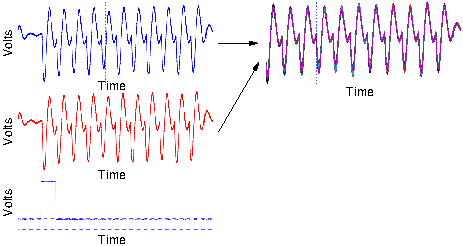
\includegraphics[scale=2.4]{../figures/tracealingment} 
		\end{figure}x150 pixel, 72dpi, 7.05x5.29 cm, bb=0 0 200 150
                    \end{center}
                \end{minipage}
                \begin{minipage}[!t]{0.39\textwidth}
                     \hspace{3ex}
                \end{minipage}
                \begin{minipage}[!t]{0.30\textwidth}
    		    \centering
                        \href{https://www.gmu.edu/}{www.gmu.edu} % Thick horizontal line
                \end{minipage}
            \end{minipage}
            %\href{http://cryptography.gmu.edu}{http://cryptography.gmu.edu} % Thick horizontal line
        \endgroup
        \clearpage
        \newcommand\blankpage{%
        \null
        \thispagestyle{empty}%
        \addtocounter{page}{-1}%
        \newpage}
        }
%\title{\Large{\textbf{Interface for Lightweight Implementations of \\Authenticated Cipher}}}
%\author{Panasayya Yalla \\ George Mason University}
%\date{}

%----------------------------------------------------------------------------------------
%   END OF TITLE PAGE
%----------------------------------------------------------------------------------------

%----------------------------------------------------------------------------------------
%   GLOSSARY 
%----------------------------------------------------------------------------------------

%----------------------------------------------------------------------------------------
%   END OF GLOSSARY
%------------------------------------------------------


%----------------------------------------------------------------------------------------
%   START OF DOCUMENT
%----------------------------------------------------------------------------------------


%----------------------------------------------------------------------------------------
%   Title Page
%----------------------------------------------------------------------------------------
\begin{document}
%%%%%%%%%%%%%%%%%%%%%%%%%%%%%%%%


%\pagenumbering{alph}
    %\maketitle
 { %\pagenumbering{gobble}
\thispagestyle{empty}
\titleAT % This command includes the title page
 \clearpage
 }
%%%%%%%%%%%%%%%%%%%%%%%%%%%%%%%%%%%%%%%%%%%%%%%%%%%%%%%%%%%%%%%%%%%%%%%%%%%%%%%%
{\pagenumbering{roman}
{\tableofcontents
%\clearpage
%\begin{appendix}
 \listoffigures
 \listoftables
 %%%%%%%%%%%%%%%%%%%%%%%%%%%%%55
 %PRINTING GLOSSARIES
 \newglossaryentry{SCA}
{
	name=SCA,
	description={Side Channel Attack}
}

\newglossaryentry{HD}
{
	name=HD,
	description={Hamming Distance}
}

\newglossaryentry{HW}
{
	name=HW,
	description={Hamming Weight}
}
 \printglossaries
 %%%%%%%%%%%%%%%%%%%%%%%%%%%%%%%5
  
%\end{appendix}
}}
%%%%%%%%%%%%%%%%%%%%%%%%%%%%%%%%%%%%%%%%%%%%%%%%%%%%%%%%%%%%%%%%%%%%%%%%%%%%%%%%
%\newglossaryentry{pdi}{name=pdi, description={Coordinated Universal Time}}
%\newglossaryentry{adt}{name=ADT, description={Atlantic Daylight Time}}
%\newglossaryentry{est}{name=EST, description={Eastern Standard Time}}
%\printglossaries
%\clearpage
%%%%%%%%%%%%%%%%%%%%%%%%%%%%%%%%%%%%%%%%%%%%%%%%%%%%%%%%%%%%%%%%%%%%%%%%%%%%%%%

\startofchapters
%\pagestyle{plain}
\chapter{Side Channel Analysis}
\section{Introduction}% to Side-Channel Analysis}
Recent years have seen a dramatic increase of market adoption and utility of so called "smart" devices
by people from all walks of life. These devices play a central role in how people are entertained, communicate,
network, work, bank and shop. Yet for every positive outcome from these devices, there is often a corollary risk.
For example, let us consider a smart phone. On one hand, there are billions of applications which provide 
unprecedented ease of access to a plethora of applications or simply termed \emph{apps} to meet any user requirements. 
On the other hands, they are also are providing a fertile environment for the distribution of hostile apps or malware.
Also, the increased power of these smart phones makes them more suitable for a host of business purposes, which can also result
in the exposure and compromise of corporate data and systems. Finally, the very portability of mobile devices means that
they are highly susceptible to loss and theft. Thus there is great need in protecting information accessed by these devices
and this information is usually secured using cryptographic algorithms. 

According to Kerchoff's Law (or Shannon's Maxim)~\cite{klaws}, \newline
\parbox[c]{\textwidth}{\textit{a cryptosystem's security must be solely based on the 
		secret key even if everything about the underlying encryption algorithm is public knowledge.}} 
However, physical implementations in hardware as well as in software 
of such encryption algorithms have been shown to
leak secret information in the form of so called side-channels
and also during sudden change in operational characteristics of the crypto-device 
i.e. via \emph{Fault Injection}. The side-channel leakage could be in the 
form of power consumption~\cite{694}, electro magnetic radiation~\cite{811} or timing~\cite{694} 
of the device. The side-channels leak sensitive information whenever the device performs an 
operation using the secret data. Attacks which make use of such inhAnalysiserent physical leakage are called 
side-channel attacks \Gls{SCA}. \Gls{SCA} is a new research area of applied cryptanalysis that has
gained popularity since mid nineties. The research in this area shows that \Gls{SCA} pose a major 
threat because the physical implementations of the cryptographic
devices are difficult to control and often result in unintended leakage of information.
Generally, all hardware implementations of cryptographic algorithms are assumed to be vulnerable to side 
channel cryptanalysis, if there are no special precautions in the implementation.

\section{Power Analysis}
   \subsection{Simple Power Analysis (SPA)}
   \subsection{Differential/Correlation Power Analysis (DPA/CPA)}
       \subsubsection{Difference of Means}
        \subsubsection{Spearman Rank Coefficient}
        \subsubsection{Pearson's r}
      
   \subsection{Power Model}
%      \begin{itemize}
     \subsubsection{Hamming Distance (HD)}
     Hamming Distance \Gls{HD}
      \subsubsection{Hamming Weight (HW)}
      Hamming Weight \Gls{HW}
 %     \end{itemize}
/nhome/aabdulga/Documents/docs/UserGuide/fobos-overview.tex
\chapter{Data Acquisition} \label{chap:dataAcquisition}

After test vectors have been generated, user can run dataAcquisition.py. The PC will send one test vector at a time to the control board, which sends it to DUT. 
The control board will trigger the oscilloscope to capture the power trace. The process will be repeated unitl all traces are collected.
 

The DUT Wrapper uses the header information in the test vector to put the data (plaintext, key etc.) into the correct FIFOs. 
The DUT Wrapper then allows the DUT (victim) algorithm to run by setting the victim reset to zero. The victim then drains the FIFOs (sdi,pdi and rdi FIFOs) and stores the output in the dout FIFO. 
Once the dout FIFO accumulates the expected amount of data, the DUT wrapper sends data to the controller which sends it to the PC.

Figure~\ref{fig:fobos-capture} shows the components of FOBOS including the handshake signals used.
Before running the \texttt{dataAcquisstion.py} script, the  user must  modify the configuration files at \texttt{config/config.txt} and \texttt{confi/acquisitionconfig.txt}.
Here is sample for \texttt{acquisitionConfig.txt} file.

\section{Data Aquisition Configuration}

\subsection{General Settings}
\begin{itemize}
 \item MEASUREMENT\_FORMAT \newline
 Possible values: dat \newline
 The format to store power measurements. Only dat is supported.
 \item LOGGING \newline 
 Possible values: INFO$|$DEBUG \newline
 The logging level. DEBUG is more verbose.
\end{itemize}

\subsection{Control Board Settings}
\begin{itemize}
 \item CONTROL\_BOARD \newline
 Possible values: Nexys3$|$Nexys2 \newline
 The Control Board type. 
 \item VICTIM\_RESET \newline
 Possible values: Integer \newline
 Reset the DUT after the specified clock cycles.
 \item TIME\_OUT \newline
 Possible values: Integer \newline
 If the DUT will not return data after the specified clock cycles, a time-out signal is returned to the PC.
\end{itemize}


\subsection{Trigger Settings}

The Control Board can send a trigger to the Oscilloscope once the DUT starts processing the data (ie. di\_ready = 0). Or it can be configured to trigger any number of clock cycles after this event occurs.
\begin{itemize}
 \item TRIGGER\_WAIT\_CYCLES \newline
 The number of clock cycles after which the trigger is asserted (after di\_ready goes to zero).
 \item TRIGGER\_LENGTH\_CYCLES \newline
 The time the trigger signal is asserted.
 \item TRIGGER\_TYPE \newline 
 possible values: TRG\_NORM, TRG\_FULL, TRG\_NORM\_CLK, TRG\_FULL\_CLK
        \begin{itemize}
          \item TRG\_NORM \newline Normal trigger mode. in this mode the TRIGGER\_WAIT\_CYCLES and TRIGGER\_LENGTH\_CYCLES are applied.
          \item TRG\_FULL \newline Full trigger mode. While DUT is running (between di\_ready = 0 and do\_valid = 1) the trigger is asserted.
          \item TRG\_NORM\_CLK \newline Similar to TRG\_NORM but the trigger signal is anded with the clock.
          \item TRG\_FULL\_CLK \newline Similar to TRG\_FULL but the trigger signal is anded with the clock.
       \end{itemize}

 \item CUT\_MODE \newline Controls how the trace retreived from the scope will be processed.
        possible values: FULL, TRIG\_HIGH
        \begin{itemize}
          \item FULL \newline The trace is cut starting at the rising edge of the trigger to the end of the screen.
          \item TRIG\_HIGH \newline the trace is cut from the rising edge to the falling edge of the trigger ie. the trace where the trigger is high will be saved.
        \end{itemize}
\end{itemize}  

\subsection{Data Settings}
\begin{itemize}
 \item DATA\_FILE \newline
 Possible values: file name (string) \newline
 The test-vector file name.
 \item EXPECTED\_OUTPUT \newline
 Possible values: Integer \newline
 Expected output size in bytes.
 \item OUTPUT\_FORMAT \newline
 Possible values: hex \newline
 Output format. 'hex' is the only supported format.
\end{itemize}

\subsection{Capture Settings}
\begin{itemize}
  \item NUMBER\_OF\_TRACES \newline
 Number of traces to collect.
 \item CAPTURE\_MODE  \newline
 Possible values: MULTI$|$SINGLE \newline
 Sigle encryption per traces or mutiple encryptions per trace.
\end{itemize}

\subsection{Oscilloscope Settings}
\begin{itemize}
 \item OSCILLOSCOPE \newline
 Possible values: AGILENT$|$OPENADC \newline
 Oscilloscope type.
 \item OSCILLOSCOPE\_IP \newline
 Possible values: IP address \newline
 Oscilloscope IP address.
 \item OSCILLOSCOPE\_PORT \newline
 Oscilloscope port number.
 \item AUTOSCALE = YES$|$NO \newline
 
 \item IMPEDANCE \newline
 Possible values: FIFTY$|$ONEMEG \newline
 Oscilloscope input impedance.
 \item CHANNELx\_RANGE  \newline
 Possible values: ON$|$OFF$|$voltage range \newline
 Oscilloscope channel voltage range (Full screen range) in Volts.
 \item TIME\_RANGE \newline
 Possible values: float (seconds)
 Oscilloscope time range in seconds (full screen time).
 \item TIMEBASE\_REF = LEFT    \newline
 \item TRIGGER\_THRESHOLD \newline
 Minimum voltage for valid trigger.
 \item TRIGGER\_SOURCE \newline
 Possible values: CHANNEL1$|$CHANNEL2$|$CHANNEL3$|$CHANNEL4 \newline
 Specifies the rigger channel.
 \item TRIGGER\_MODE =  EDGE
 \item TRIGGER\_SWEEP = NORM
 \item TRIGGER\_LEVEL = 1
 \item TRIGGER\_SLOPE = POSITIVE
 \item ACQUIRE\_TYPE = NORM$|$PEAK$|$HRES$|$AVER
 \item ACQUIRE\_MODE =  RTIM$|$ETIM$|$SEG

\end{itemize}

\section{Sample Configuration File}

\begin{verbatim}
 # ============================================= 
# Global Settings 
# ============================================= 
# ============================================= 
MEASUREMENT_FORMAT = dat # Default => dat 
LOGGING = INFO # INFO|DEBUG 
# ============================================= 
# ============================================= 
# Control Board Settings 
# ============================================= 
# ============================================= 
CONTROL_BOARD = Nexys3 
TRIGGER_WAIT_CYCLES = 0 #@VICTIM CLOCK 
TRIGGER_LENGTH_CYCLES = 1 #@VICTIM CLOCK 
TRIGGER_TYPE = TRG_FULL #TRG_NORM | TRG_FULL | TRG_NORM_CLK | TRG_FULL_CLK 
CUT_MODE = TRIG_HIGH #FULL | TRIG_HIGH 
# ============================================= 
# ============================================= 
# Test Data Generation Settings 
# ============================================= 
# ============================================= 
DATA_FILE     = dinFile.txt 
EXPECTED_OUTPUT = 16 # Expected output size in bytes 
OUTPUT_FORMAT = hex # Default => hex 
NUMBER_OF_ENCRYPTIONS_PER_TRACE = 1 
BLOCK_SIZE = 16 # In Bytes 
# ============================================= 
# ============================================= 
# FOBOS Capture Settings 
# ============================================= 
# ============================================= 
DUMMY_RUN = NO #YES/NO 
NUMBER_OF_TRACES = 50000 
#################################################### 
######## Signal Alignment Module Parameters ######## 
#################################################### 
CAPTURE_MODE = SINGLE # MULTI|SINGLE 
TRIGGER_THRESHOLD = 1.0 
# ============================================= 
# ============================================= 
# FOBOS Oscilloscope Settings 
# ============================================= 
# ============================================= 
# INTIALIZATION OPTIONS 
OSCILLOSCOPE = AGILENT #AGILENT|OPENADC 
OSCILLOSCOPE_IP = 192.168.10.10 
OSCILLOSCOPE_PORT = 5025 
AUTOSCALE = NO # YES|NO
IMPEDANCE = ONEMEG #FIFTY|ONEMEG 
# VOLTAGE AND TIME RANGE OPTIONS
CHANNEL1_RANGE = 0.060V 
CHANNEL2_RANGE = 6V 
CHANNEL3_RANGE = OFF # ON|OFF|voltage range 
CHANNEL4_RANGE = OFF # ON|OFF|voltage range 
TIME_RANGE = 0.000050 
TIMEBASE_REF = LEFT
# TRIGGER OPTIONS 
TRIGGER_SOURCE = CHANNEL2 
TRIGGER_MODE = EDGE
TRIGGER_SWEEP = NORM 
TRIGGER_LEVEL = 1 
TRIGGER_SLOPE = POSITIVE 
# ACQUIRE OPTIONS 
ACQUIRE_TYPE = NORM # NORM|PEAK|HRES|AVER 
ACQUIRE_MODE = RTIM # RTIM | ETIM| SEG
\end{verbatim}

\section{Running Data Acquisition}
Once the configuration is done, user can run 

\texttt{python dataAcquisition.py }

The output will be saved in \texttt{workspace/$<$projectName$>$/measurements}. The traces are stored in a Numpy array called \texttt{rawDataAligned.npy}.





\chapter{FOBOS Analysis}
\section{Power Model}
\section{Trace Alignment}
\section{Sample Window}
\section{Compression}
\section{Example}
\section{Files}
%\begin{figure}
%label=\fbox{\color{Black}data.txt},
%labelposition=topline,
%\VerbatimInput{./files/dataAnalysisParams.txt}
%\end{figure}
\begin{tcolorbox}[colback=yellow!10!white,colframe=green!75!black,title=dataAnalysisParams.txt]
	\textbf{Location:}fobos/bin/config/dataAnalysisParams.txt
	\tcblower
	\footnotesize
	\verbatiminput{./files/dataAnalysisParams.txt}
	\label{file:1}
\end{tcolorbox}
\begin{tcolorbox}[colback=yellow!10!white,colframe=green!75!black,title=compressionParams.txt]
	\textbf{Location:}fobos/bin/config/compressionParams.txt
	\tcblower
	\footnotesize
	\verbatiminput{./files/compressionParams.txt}
	\label{file:1}
\end{tcolorbox}
\begin{tcolorbox}[colback=yellow!10!white,colframe=green!75!black,title=postProcessesParams.txt]
	\textbf{Location:}fobos/bin/config/postProcessesParams.txt
	\tcblower
	\footnotesize
	\verbatiminput{./files/postProcessesParams.txt}
	\label{file:1}
\end{tcolorbox}
\begin{tcolorbox}[colback=yellow!10!white,colframe=green!75!black,title=projectPath.txt]
	\textbf{Location:}fobos/bin/config/projectPath.txt
	\tcblower
	\footnotesize
	\verbatiminput{./files/projectPath.txt}
	\label{file:1}
\end{tcolorbox}
\begin{tcolorbox}[colback=yellow!10!white,colframe=green!75!black,title=sampleSpaceDispParams.txt]
	\textbf{Location:}fobos/bin/config/sampleSpaceDispParams.txt
	\tcblower
	\footnotesize
	\verbatiminput{./files/sampleSpaceDispParams.txt}
	\label{file:1}
\end{tcolorbox}
\begin{tcolorbox}[colback=yellow!10!white,colframe=green!75!black,title=signalAlignmentParams.txt]
	\textbf{Location:}fobos/bin/config/signalAlignmentParams.txt
	\tcblower
	\footnotesize
	\verbatiminput{./files/signalAlignmentParams.txt}
	\label{file:1}
\end{tcolorbox}
\begin{tcolorbox}[colback=yellow!10!white,colframe=green!75!black,title=traceExpungeParams.txt]
	\textbf{Location:}fobos/bin/config/traceExpungeParams.txt
	\tcblower
	\footnotesize
	\verbatiminput{./files/traceExpungeParams.txt}
	\label{file:1}
\end{tcolorbox}

\begin{tcolorbox}[colback=yellow!10!white,colframe=green!75!black,title=config.txt]
	\textbf{Location:}fobos/bin/config/config.txt
	\tcblower
	\footnotesize
	\verbatiminput{./files/config.txt}
	\label{file:1}
\end{tcolorbox}

%\verbatiminput{./files/dataAnalysisParams.txt}


%%%%%%%%%%%%%%%%%%%%%%%%%%%%%%%%


%\pagenumbering{alph}
    %\maketitle
 { %\pagenumbering{gobble}
\thispagestyle{empty}
\titleATa % This command includes the title page
 \clearpage
 }
%%%%%%%%%%%%%%%%%%%%%%%%%%%%%%%%%%%%%%%%%%%%%%%%%%%%%%%%%%%%%%%%%%%%%%%%%%%%%%%%
{\pagenumbering{roman}
{\tableofcontents
%\clearpage
%\begin{appendix}
 \listoffigures
 \listoftables
 \newglossaryentry{SCA}
{
	name=SCA,
	description={Side Channel Attack}
}

\newglossaryentry{HD}
{
	name=HD,
	description={Hamming Distance}
}

\newglossaryentry{HW}
{
	name=HW,
	description={Hamming Weight}
}
 \printglossaries
 
%\end{appendix}
}}
%%%%%%%%%%%%%%%%%%%%%%%%%%%%%%%%%%%%%%%%%%%%%%%%%%%%%%%%%%%%%%%%%%%%%%%%%%%%%%%%
%\newglossaryentry{pdi}{name=pdi, description={Coordinated Universal Time}}
%\newglossaryentry{adt}{name=ADT, description={Atlantic Daylight Time}}
%\newglossaryentry{est}{name=EST, description={Eastern Standard Time}}
%\printglossaries
%\clearpage
%%%%%%%%%%%%%%%%%%%%%%%%%%%%%%%%%%%%%%%%%%%%%%%%%%%%%%%%%%%%%%%%%%%%%%%%%%%%%%%

\startofchapters
%\pagestyle{plain}
%\chapter{Side Channel Analysis}
\section{Introduction}% to Side-Channel Analysis}
Recent years have seen a dramatic increase of market adoption and utility of so called "smart" devices
by people from all walks of life. These devices play a central role in how people are entertained, communicate,
network, work, bank and shop. Yet for every positive outcome from these devices, there is often a corollary risk.
For example, let us consider a smart phone. On one hand, there are billions of applications which provide 
unprecedented ease of access to a plethora of applications or simply termed \emph{apps} to meet any user requirements. 
On the other hands, they are also are providing a fertile environment for the distribution of hostile apps or malware.
Also, the increased power of these smart phones makes them more suitable for a host of business purposes, which can also result
in the exposure and compromise of corporate data and systems. Finally, the very portability of mobile devices means that
they are highly susceptible to loss and theft. Thus there is great need in protecting information accessed by these devices
and this information is usually secured using cryptographic algorithms. 

According to Kerchoff's Law (or Shannon's Maxim)~\cite{klaws}, \newline
\parbox[c]{\textwidth}{\textit{a cryptosystem's security must be solely based on the 
		secret key even if everything about the underlying encryption algorithm is public knowledge.}} 
However, physical implementations in hardware as well as in software 
of such encryption algorithms have been shown to
leak secret information in the form of so called side-channels
and also during sudden change in operational characteristics of the crypto-device 
i.e. via \emph{Fault Injection}. The side-channel leakage could be in the 
form of power consumption~\cite{694}, electro magnetic radiation~\cite{811} or timing~\cite{694} 
of the device. The side-channels leak sensitive information whenever the device performs an 
operation using the secret data. Attacks which make use of such inhAnalysiserent physical leakage are called 
side-channel attacks \Gls{SCA}. \Gls{SCA} is a new research area of applied cryptanalysis that has
gained popularity since mid nineties. The research in this area shows that \Gls{SCA} pose a major 
threat because the physical implementations of the cryptographic
devices are difficult to control and often result in unintended leakage of information.
Generally, all hardware implementations of cryptographic algorithms are assumed to be vulnerable to side 
channel cryptanalysis, if there are no special precautions in the implementation.

\section{Power Analysis}
   \subsection{Simple Power Analysis (SPA)}
   \subsection{Differential/Correlation Power Analysis (DPA/CPA)}
       \subsubsection{Difference of Means}
        \subsubsection{Spearman Rank Coefficient}
        \subsubsection{Pearson's r}
      
   \subsection{Power Model}
%      \begin{itemize}
     \subsubsection{Hamming Distance (HD)}
     Hamming Distance \Gls{HD}
      \subsubsection{Hamming Weight (HW)}
      Hamming Weight \Gls{HW}
 %     \end{itemize}
/nhome/aabdulga/Documents/docs/UserGuide/fobos-overview.tex
\chapter{Data Acquisition} \label{chap:dataAcquisition}

After test vectors have been generated, user can run dataAcquisition.py. The PC will send one test vector at a time to the control board, which sends it to DUT. 
The control board will trigger the oscilloscope to capture the power trace. The process will be repeated unitl all traces are collected.
 

The DUT Wrapper uses the header information in the test vector to put the data (plaintext, key etc.) into the correct FIFOs. 
The DUT Wrapper then allows the DUT (victim) algorithm to run by setting the victim reset to zero. The victim then drains the FIFOs (sdi,pdi and rdi FIFOs) and stores the output in the dout FIFO. 
Once the dout FIFO accumulates the expected amount of data, the DUT wrapper sends data to the controller which sends it to the PC.

Figure~\ref{fig:fobos-capture} shows the components of FOBOS including the handshake signals used.
Before running the \texttt{dataAcquisstion.py} script, the  user must  modify the configuration files at \texttt{config/config.txt} and \texttt{confi/acquisitionconfig.txt}.
Here is sample for \texttt{acquisitionConfig.txt} file.

\section{Data Aquisition Configuration}

\subsection{General Settings}
\begin{itemize}
 \item MEASUREMENT\_FORMAT \newline
 Possible values: dat \newline
 The format to store power measurements. Only dat is supported.
 \item LOGGING \newline 
 Possible values: INFO$|$DEBUG \newline
 The logging level. DEBUG is more verbose.
\end{itemize}

\subsection{Control Board Settings}
\begin{itemize}
 \item CONTROL\_BOARD \newline
 Possible values: Nexys3$|$Nexys2 \newline
 The Control Board type. 
 \item VICTIM\_RESET \newline
 Possible values: Integer \newline
 Reset the DUT after the specified clock cycles.
 \item TIME\_OUT \newline
 Possible values: Integer \newline
 If the DUT will not return data after the specified clock cycles, a time-out signal is returned to the PC.
\end{itemize}


\subsection{Trigger Settings}

The Control Board can send a trigger to the Oscilloscope once the DUT starts processing the data (ie. di\_ready = 0). Or it can be configured to trigger any number of clock cycles after this event occurs.
\begin{itemize}
 \item TRIGGER\_WAIT\_CYCLES \newline
 The number of clock cycles after which the trigger is asserted (after di\_ready goes to zero).
 \item TRIGGER\_LENGTH\_CYCLES \newline
 The time the trigger signal is asserted.
 \item TRIGGER\_TYPE \newline 
 possible values: TRG\_NORM, TRG\_FULL, TRG\_NORM\_CLK, TRG\_FULL\_CLK
        \begin{itemize}
          \item TRG\_NORM \newline Normal trigger mode. in this mode the TRIGGER\_WAIT\_CYCLES and TRIGGER\_LENGTH\_CYCLES are applied.
          \item TRG\_FULL \newline Full trigger mode. While DUT is running (between di\_ready = 0 and do\_valid = 1) the trigger is asserted.
          \item TRG\_NORM\_CLK \newline Similar to TRG\_NORM but the trigger signal is anded with the clock.
          \item TRG\_FULL\_CLK \newline Similar to TRG\_FULL but the trigger signal is anded with the clock.
       \end{itemize}

 \item CUT\_MODE \newline Controls how the trace retreived from the scope will be processed.
        possible values: FULL, TRIG\_HIGH
        \begin{itemize}
          \item FULL \newline The trace is cut starting at the rising edge of the trigger to the end of the screen.
          \item TRIG\_HIGH \newline the trace is cut from the rising edge to the falling edge of the trigger ie. the trace where the trigger is high will be saved.
        \end{itemize}
\end{itemize}  

\subsection{Data Settings}
\begin{itemize}
 \item DATA\_FILE \newline
 Possible values: file name (string) \newline
 The test-vector file name.
 \item EXPECTED\_OUTPUT \newline
 Possible values: Integer \newline
 Expected output size in bytes.
 \item OUTPUT\_FORMAT \newline
 Possible values: hex \newline
 Output format. 'hex' is the only supported format.
\end{itemize}

\subsection{Capture Settings}
\begin{itemize}
  \item NUMBER\_OF\_TRACES \newline
 Number of traces to collect.
 \item CAPTURE\_MODE  \newline
 Possible values: MULTI$|$SINGLE \newline
 Sigle encryption per traces or mutiple encryptions per trace.
\end{itemize}

\subsection{Oscilloscope Settings}
\begin{itemize}
 \item OSCILLOSCOPE \newline
 Possible values: AGILENT$|$OPENADC \newline
 Oscilloscope type.
 \item OSCILLOSCOPE\_IP \newline
 Possible values: IP address \newline
 Oscilloscope IP address.
 \item OSCILLOSCOPE\_PORT \newline
 Oscilloscope port number.
 \item AUTOSCALE = YES$|$NO \newline
 
 \item IMPEDANCE \newline
 Possible values: FIFTY$|$ONEMEG \newline
 Oscilloscope input impedance.
 \item CHANNELx\_RANGE  \newline
 Possible values: ON$|$OFF$|$voltage range \newline
 Oscilloscope channel voltage range (Full screen range) in Volts.
 \item TIME\_RANGE \newline
 Possible values: float (seconds)
 Oscilloscope time range in seconds (full screen time).
 \item TIMEBASE\_REF = LEFT    \newline
 \item TRIGGER\_THRESHOLD \newline
 Minimum voltage for valid trigger.
 \item TRIGGER\_SOURCE \newline
 Possible values: CHANNEL1$|$CHANNEL2$|$CHANNEL3$|$CHANNEL4 \newline
 Specifies the rigger channel.
 \item TRIGGER\_MODE =  EDGE
 \item TRIGGER\_SWEEP = NORM
 \item TRIGGER\_LEVEL = 1
 \item TRIGGER\_SLOPE = POSITIVE
 \item ACQUIRE\_TYPE = NORM$|$PEAK$|$HRES$|$AVER
 \item ACQUIRE\_MODE =  RTIM$|$ETIM$|$SEG

\end{itemize}

\section{Sample Configuration File}

\begin{verbatim}
 # ============================================= 
# Global Settings 
# ============================================= 
# ============================================= 
MEASUREMENT_FORMAT = dat # Default => dat 
LOGGING = INFO # INFO|DEBUG 
# ============================================= 
# ============================================= 
# Control Board Settings 
# ============================================= 
# ============================================= 
CONTROL_BOARD = Nexys3 
TRIGGER_WAIT_CYCLES = 0 #@VICTIM CLOCK 
TRIGGER_LENGTH_CYCLES = 1 #@VICTIM CLOCK 
TRIGGER_TYPE = TRG_FULL #TRG_NORM | TRG_FULL | TRG_NORM_CLK | TRG_FULL_CLK 
CUT_MODE = TRIG_HIGH #FULL | TRIG_HIGH 
# ============================================= 
# ============================================= 
# Test Data Generation Settings 
# ============================================= 
# ============================================= 
DATA_FILE     = dinFile.txt 
EXPECTED_OUTPUT = 16 # Expected output size in bytes 
OUTPUT_FORMAT = hex # Default => hex 
NUMBER_OF_ENCRYPTIONS_PER_TRACE = 1 
BLOCK_SIZE = 16 # In Bytes 
# ============================================= 
# ============================================= 
# FOBOS Capture Settings 
# ============================================= 
# ============================================= 
DUMMY_RUN = NO #YES/NO 
NUMBER_OF_TRACES = 50000 
#################################################### 
######## Signal Alignment Module Parameters ######## 
#################################################### 
CAPTURE_MODE = SINGLE # MULTI|SINGLE 
TRIGGER_THRESHOLD = 1.0 
# ============================================= 
# ============================================= 
# FOBOS Oscilloscope Settings 
# ============================================= 
# ============================================= 
# INTIALIZATION OPTIONS 
OSCILLOSCOPE = AGILENT #AGILENT|OPENADC 
OSCILLOSCOPE_IP = 192.168.10.10 
OSCILLOSCOPE_PORT = 5025 
AUTOSCALE = NO # YES|NO
IMPEDANCE = ONEMEG #FIFTY|ONEMEG 
# VOLTAGE AND TIME RANGE OPTIONS
CHANNEL1_RANGE = 0.060V 
CHANNEL2_RANGE = 6V 
CHANNEL3_RANGE = OFF # ON|OFF|voltage range 
CHANNEL4_RANGE = OFF # ON|OFF|voltage range 
TIME_RANGE = 0.000050 
TIMEBASE_REF = LEFT
# TRIGGER OPTIONS 
TRIGGER_SOURCE = CHANNEL2 
TRIGGER_MODE = EDGE
TRIGGER_SWEEP = NORM 
TRIGGER_LEVEL = 1 
TRIGGER_SLOPE = POSITIVE 
# ACQUIRE OPTIONS 
ACQUIRE_TYPE = NORM # NORM|PEAK|HRES|AVER 
ACQUIRE_MODE = RTIM # RTIM | ETIM| SEG
\end{verbatim}

\section{Running Data Acquisition}
Once the configuration is done, user can run 

\texttt{python dataAcquisition.py }

The output will be saved in \texttt{workspace/$<$projectName$>$/measurements}. The traces are stored in a Numpy array called \texttt{rawDataAligned.npy}.





\chapter{FOBOS Analysis}
\section{Power Model}
\section{Trace Alignment}
\section{Sample Window}
\section{Compression}
\section{Example}
\section{Files}
%\begin{figure}
%label=\fbox{\color{Black}data.txt},
%labelposition=topline,
%\VerbatimInput{./files/dataAnalysisParams.txt}
%\end{figure}
\begin{tcolorbox}[colback=yellow!10!white,colframe=green!75!black,title=dataAnalysisParams.txt]
	\textbf{Location:}fobos/bin/config/dataAnalysisParams.txt
	\tcblower
	\footnotesize
	\verbatiminput{./files/dataAnalysisParams.txt}
	\label{file:1}
\end{tcolorbox}
\begin{tcolorbox}[colback=yellow!10!white,colframe=green!75!black,title=compressionParams.txt]
	\textbf{Location:}fobos/bin/config/compressionParams.txt
	\tcblower
	\footnotesize
	\verbatiminput{./files/compressionParams.txt}
	\label{file:1}
\end{tcolorbox}
\begin{tcolorbox}[colback=yellow!10!white,colframe=green!75!black,title=postProcessesParams.txt]
	\textbf{Location:}fobos/bin/config/postProcessesParams.txt
	\tcblower
	\footnotesize
	\verbatiminput{./files/postProcessesParams.txt}
	\label{file:1}
\end{tcolorbox}
\begin{tcolorbox}[colback=yellow!10!white,colframe=green!75!black,title=projectPath.txt]
	\textbf{Location:}fobos/bin/config/projectPath.txt
	\tcblower
	\footnotesize
	\verbatiminput{./files/projectPath.txt}
	\label{file:1}
\end{tcolorbox}
\begin{tcolorbox}[colback=yellow!10!white,colframe=green!75!black,title=sampleSpaceDispParams.txt]
	\textbf{Location:}fobos/bin/config/sampleSpaceDispParams.txt
	\tcblower
	\footnotesize
	\verbatiminput{./files/sampleSpaceDispParams.txt}
	\label{file:1}
\end{tcolorbox}
\begin{tcolorbox}[colback=yellow!10!white,colframe=green!75!black,title=signalAlignmentParams.txt]
	\textbf{Location:}fobos/bin/config/signalAlignmentParams.txt
	\tcblower
	\footnotesize
	\verbatiminput{./files/signalAlignmentParams.txt}
	\label{file:1}
\end{tcolorbox}
\begin{tcolorbox}[colback=yellow!10!white,colframe=green!75!black,title=traceExpungeParams.txt]
	\textbf{Location:}fobos/bin/config/traceExpungeParams.txt
	\tcblower
	\footnotesize
	\verbatiminput{./files/traceExpungeParams.txt}
	\label{file:1}
\end{tcolorbox}

\begin{tcolorbox}[colback=yellow!10!white,colframe=green!75!black,title=config.txt]
	\textbf{Location:}fobos/bin/config/config.txt
	\tcblower
	\footnotesize
	\verbatiminput{./files/config.txt}
	\label{file:1}
\end{tcolorbox}

%\verbatiminput{./files/dataAnalysisParams.txt}

 

\end{document}
